%%%%%%%%%%%%%%%%%%%%%%%%%%%%%%%%%%%%%%%%%%%%%%%%%%%%%%%%%%%%%%%%%%%
%%%%%%%%%%%%%%%%%%%%%%%%%%%%%%%%%%%%%%%%%%%%%%%%%%%%%%%%%%%%%%%%%%%
% Описание "графа" процессов
%%%%%%%%%%%%%%%%%%%%%%%%%%%%%%%%%%%%%%%%%%%%%%%%%%%%%%%%%%%%%%%%%%%
%%%%%%%%%%%%%%%%%%%%%%%%%%%%%%%%%%%%%%%%%%%%%%%%%%%%%%%%%%%%%%%%%%%

Представление графа процессов в Haskell затруднено тем, что графовые
структуры данных обычно требуют ссылок на произвольные узлы,
что приводит к появлению перекрёсных ссылок. Прямая реализация этой
идеи сложна в разработке и поддержке и не является идиоматичной.
Использование \emph{IORef}\footnote{https://hackage.haskell.org/package/base-4.11.1.0/docs/Data-IORef.html},
хотя и предоставляет мутабельность, приводит к неоправданному усложнению кода всего проекта,
избавляя код от функциональной чистоты.

Заметим, что графовость этой структуре данных придают \emph{обратные рёбра}
(то есть рёбра от детей к родителям), которые появляются при свёртке, когда ребёнок
является переименованием родителя.
Тогда, если уметь сохранять или восстанавливать информацию об этой связи, то
достаточным будет представить граф в качестве \emph{дерева} процессов.
Древовидные структура однозначно отображается на процесс символьных вычислений,
а также они легко и идиоматично в Haskell.

Структура дерева процессов представлена в виде дерева на рисунке~\ref{fig:ptree}.

\begin{figure}[h!]
\begin{lstlisting}[mathescape,language=Haskell,extendedchars=\true,frame=single,basicstyle=\ttfamily]

type Conf = Conjunction (RelationCall FreeVar)

type Subs = Variable $\mapsto$ Term

data Tree where
  Failure     :: Tree
  Success     :: Subst $\rarrow$ Tree
  Renaming    :: Conf $\rarrow$ Subst $\rarrow$ Tree
  Abstraction :: Conf $\rarrow$ Subst $\rarrow$ List Tree $\rarrow$ Tree
  Generalizer :: Subst $\rarrow$ Tree $\rarrow$ Tree
  Unfolding   :: Conf $\rarrow$ Subst $\rarrow$ List Tree $\rarrow$ Tree
\end{lstlisting}
\caption{Описание дерева процессов.}
\label{fig:ptree}
\end{figure}

Конфигурация \lstinline{Conf} определена как выражение со свободными переменными.
В узле дерева процессов хранится конфигурация, приведённая к форме, содержащей только конъюнкцию вызовов
реляционного отношения. Это сделано из тех соображений, что, во-первых, дизъюнкция представляет
собой ветвление вычислений, посему, соответственно, представляется как ветвление в дереве процессов,
во-вторых, унификации производятся во время символьных вычислений и добавляются в подстановку,
в-третьих, так как введение свежей переменной оказывает влияние лишь на состояние, в котором производятся вычисления,
неосмысленно сохранять его в конфигурации.

Подстановка \lstinline{Subst} соответствует своему математическому определению как отображению из
переменных в термы.
Узлы дерева процессов представляют шаги суперкомпиляции и исходы вычисления выражений:
\begin{itemize}
\item \lstinline{Failure} обозначает неудавшееся вычисления. Такой исход
      случается при появлении противоречивых подстановок;
\item \lstinline{Success}, напротив, обозначает удавшееся вычисление, которое свелось к подстановке \lstinline{Subst};
\item \lstinline{Renaming} обозначает узел, конфигурация которой является переименованием какого-то родительского узла.
\item \lstinline{Abstraction} обознает узел, который может быть обобщён на одного из родителей.
      После обобщения может появится несколько конфигураций, которые являются результатом применения разделения.
      Эти конфигурации добавляются в качестве списка дочерних поддеревьев в текущий узел. 
\item \lstinline{Generalizer} \todo{описать после того, как опишешь обобщение}
\item \lstinline{Unfolding} обознает шаг символьного вычисления, на котором  
\end{itemize}

%%%%%%%%%%%%%%%%%%%%%%%%%%%%%%%%%%%%%%%%%%%%%%%%%%%%%%%%%%%%%%%%%%%
%%%%%%%%%%%%%%%%%%%%%%%%%%%%%%%%%%%%%%%%%%%%%%%%%%%%%%%%%%%%%%%%%%%
% Описание окружения
%%%%%%%%%%%%%%%%%%%%%%%%%%%%%%%%%%%%%%%%%%%%%%%%%%%%%%%%%%%%%%%%%%%
%%%%%%%%%%%%%%%%%%%%%%%%%%%%%%%%%%%%%%%%%%%%%%%%%%%%%%%%%%%%%%%%%%%

\emph{Окружение} для суперкомпиляции должно сохранять следующие объекты:
\begin{itemize}
\item подстановку, в которой содержатся все накопленные непротиворечивые унификации,
      необходимую в процессе прогонки для проверки новых унификаций;
\item первую свободную семантическую переменную, необходимую для генерации свежих переменных,
      к примеру, при абстракции;
\item определение программы, необходимое для замены вызова на своё тело.
\end{itemize}

\todo{Что-то ещё об этом нужно написать!}

%%%%%%%%%%%%%%%%%%%%%%%%%%%%%%%%%%%%%%%%%%%%%%%%%%%%%%%%%%%%%%%%%%%
%%%%%%%%%%%%%%%%%%%%%%%%%%%%%%%%%%%%%%%%%%%%%%%%%%%%%%%%%%%%%%%%%%%
% Описание шага unfolding'а
%%%%%%%%%%%%%%%%%%%%%%%%%%%%%%%%%%%%%%%%%%%%%%%%%%%%%%%%%%%%%%%%%%%
%%%%%%%%%%%%%%%%%%%%%%%%%%%%%%%%%%%%%%%%%%%%%%%%%%%%%%%%%%%%%%%%%%%

Шаг символьного вычисления по данной конфигурации $C$ порождает
множество конфигурации $\{ C_1, \dots, C_n \}$, описывающих состояния в которое может перейти
процесс реального исполнения программы. Классически, шаг символьного
вычисления соответствует семантике языка, который суперкомпилируется,
и для \ukanren существует сертифицированная семантика\cite{semanticMK},
однако описание шага символьного вычисления \ukanren для суперкомпиляции 
усложнено тем, что реляционные языки не исполняются привычным образом,
как, к примеру, функциональные программы, и \emph{поиск}, вшитый в семантику,
не ложится на суперкомпиляцию.

Тогда порождённую конфигурацию можно рассматривать не как непосредственный
шаг вычисления, но как возможное состояние, в которое может перейти программа.
Такое состояние появляется путём раскрытия тела одного или нескольких
конъюнктов конфигурации.

К примеру, рассмотрим часть программы на \ukanren на рисунке~\ref{fig:unfoldEx}, в котором
определены какие-то отношения \lstinline{f} и \lstinline{g}.
\begin{figure}[h!]
\begin{lstlisting}
f(a) = f'(a)$\lor$f''(a)
g(a, b) = g'(a)$\land$g''(b)
\end{lstlisting}
\caption{Пример отношений для демонстрации шага символьных вычислений}
\label{fig:unfoldEx}
\end{figure}

Допустим, на шаге суперкомпиляции алгоритм обрабаывает конфигурацию
\lstinline{f($\text{v}_\text{1}$)$\land$g($\text{v}_\text{1}$, $\text{v}_\text{2}$)}
хотим сделать шаг символьного вычисления. Рассмотрим несколько способов породить новые конфигурации.
\begin{itemize}
\item Если раскроется определение \lstinline{f}, то будут получены новые конфигурации 
      \lstinline{f'($\text{v}_\text{1}$)$\land$g($\text{v}_\text{1}$, $\text{v}_\text{2}$)} и
      \lstinline{f''($\text{v}_\text{1}$)$\land$g($\text{v}_\text{1}$, $\text{v}_\text{2}$)}.
\item Если раскроется определение \lstinline{g}, то будет получена новая конфигурация 
      \lstinline{f($\text{v}_\text{1}$)$\land$g'($\text{v}_\text{1}$)$\land$g''($\text{v}_\text{2}$)}.
\item Если раскроются оба определения \lstinline{f} и \lstinline{g}, то будут получены новые конфигурации 
      \lstinline{f'($\text{v}_\text{1}$)$\land$g($\text{v}_\text{1}$)$\land$g''($\text{v}_\text{2}$)} и
      \lstinline{f''($\text{v}_\text{1}$)$\land$g($\text{v}_\text{1}$)$\land$g''($\text{v}_\text{2}$)}.
\end{itemize}

Последний набор конфигураций --- это полный набор состояний, в которые процесс вычислений может
прийти. В первых двух наборах, можно отметить, порождённые конфигурации не исключают
возможные состояния процессов, отображённые в последнем наборе, они могут появится на последующих шагах вычисления,
если перед этим ветвь исполнения не будет остановлена из-за противоречивой подстановки.

Таким образом, какой-бы способ развёртывания определений не был бы выбран, он не будет
исключать состояния, в которые процесс вычисления теоретически может прийти, но выбор
разных стратегий развёртывания может систематически приводить к разным деревьям процессов,
а следовательно, приводить к различным эффектам специализации.

Базовой стратегией порождения новых конфигураций выбрана \emph{полная стратегия развёртывания},
пример которой был показан выше, при которой мы заменяем определния всех реляционных вызовов
конфигурации.

%%%%%%%%%%%%%%%%%%%%%%%%%%%%%%%%%%%%%%%%%%%%%%%%%%%%%%%%%%%%%%%%%%%
%%%%%%%%%%%%%%%%%%%%%%%%%%%%%%%%%%%%%%%%%%%%%%%%%%%%%%%%%%%%%%%%%%%
% Описание общего алгоритма суперкомпиляции
%%%%%%%%%%%%%%%%%%%%%%%%%%%%%%%%%%%%%%%%%%%%%%%%%%%%%%%%%%%%%%%%%%%
%%%%%%%%%%%%%%%%%%%%%%%%%%%%%%%%%%%%%%%%%%%%%%%%%%%%%%%%%%%%%%%%%%%

\subsubsection{Обобщённый алгоритм суперкомпиляции}

Обобщённый алгоритм суперкомпиляции представлен на рисунке~\ref{fig:scalgogen}.
\todo{Подробнее:)}

\begin{figure}[h!]
\begin{lstlisting}[mathescape,language=Haskell,extendedchars=\true,frame=single,basicstyle=\ttfamily]
drive(env, tree, expression):
  if expression is empty
  then add(env, tree, success node)
  else if $\exists \text{parent}:$ expression is renaming of parent
  then add(env, tree, renaming node)
  $\text{\color{red}TODO: Ввести нотацию для } \embed^+$
  else if $\exists$ parent: parent $\embed^+$ expression
  then
     node $\larrow$ abstractUp(expression, parent)
     addUp(env, tree, parent, node)
  else else if $\exists$ parent: parent $\embed^*$ expression
  then
    add(abstraction, node)
    children $\larrow$ abstract(expression, parent)
    $\forall \text{child} \in \text{children}:$
      drive(tree, child)
  else
    add(unfolding node)
    children $\larrow$ unfold(expression)
    $\forall \text{child} \in \text{children}:$
      drive(tree, child)
\end{lstlisting}
\caption{Обобщённый алгоритм суперкомпиляции}
\label{fig:scalgogen}
\end{figure}


%%%%%%%%%%%%%%%%%%%%%%%%%%%%%%%%%%%%%%%%%%%%%%%%%%%%%%%%%%%%%%%%%%%
%%%%%%%%%%%%%%%%%%%%%%%%%%%%%%%%%%%%%%%%%%%%%%%%%%%%%%%%%%%%%%%%%%%
% Описание конкретного алгоритма суперкомпиляции
%%%%%%%%%%%%%%%%%%%%%%%%%%%%%%%%%%%%%%%%%%%%%%%%%%%%%%%%%%%%%%%%%%%
%%%%%%%%%%%%%%%%%%%%%%%%%%%%%%%%%%%%%%%%%%%%%%%%%%%%%%%%%%%%%%%%%%%
\subsubsection{Конкретный алгоритм суперкомпиляции}

Наличие операции обобщения вверх предполагает, что необходимо умение передвигаться по дереву вверх и изменять его. 
Реализация в Haskell этой идеи --- задача крайне нетривиальная. Возможно представлять
деревья в мутабельных массивах, однако при обобщении необходимо удалять целые поддеревья,
что при таком подходе сложная операция.

Классическим способом решения этой проблемы являются \emph{зипперы}\cite{zipper}.
Эта идиома предлагает рассматривать структуру данных как пару из элемента,
на котором установлен фокус, и контекста, который представляется как структура данных
с ``дыркой'', в котором сфокусированный элемент должен находиться.

К примеру, зиппер для списка \lstinline{[1, 2, 3, 4]} при фокусе на 3 представляется
таким образом: \lstinline{(3, ([2, 1, 0], [4, 5, 6]))}.
Тогда перефокусировка вправо или влево на один элемент происходит за константу,
как и замена элемента, для которой достаточно заменить первую компоненту пары.
В то время как, в силу того, что операция взятия элемента в связном списке по индексу
происходит за линейное время от длины списка, взятие элемента слева от 3 также
будет происходить за линейное время, как и, соответственно, модификация списка.

Для деревьев с произвольным количеством детей зиппер может выглядеть
как пара из текущего узла и списка родителей, отсортированного в порядке
близости к узлу (рисунок~\ref{fig:zipper}). 
\begin{figure}[h!]
\begin{lstlisting}[mathescape,language=Haskell,extendedchars=\true,frame=single,basicstyle=\ttfamily]
data Parent = Parent { children :: ListZipper Node }
type TreeZipper = (Node, List Parent)
\end{lstlisting}
\caption{Пример структуры зиппера для деревьев}
\label{fig:zipper}
\end{figure}

Родительский (структура \lstinline{Parent}) cписок детей представлен в виде зиппера (поле \lstinline{children})
для списка, в котором происходит фокус: у непосредственного родителя --- на элемент в фокусе, а у остальных
родителей --- на предыдущего в порядке сортировки.\todo{more?}

При представлении дерева процессов в идиоме зипперов основа алгоритма суперкомпиляции
принимает форму описания действий при смене состояния зиппера.
\todo{TODO}

\subsubsection{Модификации базового алгоритма суперкомпиляции}

\paragraph{Поиск узлов для переименования среди всех вычисленных поддеревьев}\ \\
В базовом алгоритме суперкомпиляции поиск узлов на которые происходят переименования происходит
среди родителей. Это напрямую соотносится с понятием символьных вычислений: по достижении
узла, которое является переименованием уже встреченного, вычисление переходит на родительский узел.
Однако довольно части встречается, что в разных поддеревьях дерева процессов стречаются одинаковые
конфигурации, поддеревья которых оказываются полностью идентичными. В таком случае, кажется
очевидной оптмизация, при которой мы запоминаем вычисленные поддеревья и в случае,
когда мы встречаем схожу конфигурацию, не вычисляем поддерево заново, добавляя ссылку на него.
\todo{Показать, почему это ничего не сломает}

\paragraph{Стратегии развёртывания реляционных вызовов}\ \\
Как уже говорилось, разные стратегии развёртывания реляционных вызовов могут привести к разным
эффектам специализации. К примеру, полная стратегия развёртывания, которая была принята за базовую,
приводит к \emph{таплингу} \origin{tupling}\cite{tupling} --- оптмизации, при которой
множество проходов по одной структуре данных заменяется на один проход.

% Может, показать, что оно круто всё строит?

Основной недостаток базового подхода в том, что он для получения всех возможных состояний
производит декартово производение тел вызовов в конъюнкциях, что приводит
к сильному разрастанию дерева процессов и, как следствия, сильно требователен к вычислительным ресурсам.
Вследствие чего реализация новых стратегий развёртывания производится не только в исследовательских,
но и прикладных целях.

Для лёгкой подмены стратегий суперкомпиляции был разработан специальный интерфейс \lstinline{UnfoldableGoal}
(рисунок~\ref{fig:unfoldable}).
\begin{figure}[h!]
\begin{lstlisting}
class Unfoldable a where
   initialize :: Conf $\rarrow$ a
   get        :: a $\rarrow$ Conf
   unfoldStep :: a $\rarrow$ Env $\rarrow$ List (Env, a)
\end{lstlisting}
\caption{Интерфейс для различных стратегий развёртывания.}
\label{fig:unfoldable}
\end{figure}

Предоставляемые интерфейсом функции используются в алгоритме суперкомпиляции следующим образом:
\begin{itemize}
\item \lstinline{initialize} оборачивает конфигурацию в структуру, в которой может содержаться
      вспомогательная информация для процесса развёртывания;
\item \lstinline{get} позволяет получить конфигурацию для применения её к операциям, не зависящим
      от стратегий;
\item \lstinline{unfoldStep} непосредственно проводит шаг вычисления на основе текущей конфигурации
      и её окружения, порождая новые конфигурации с соответствующими им состояниями.
\end{itemize}

В работе рассмотрен и реализован ряд стратегий, описанные ниже.

\begin{itemize}
\item {\bf Последовательная стратегия развёртывания}, при которой отслеживается,
      какой вызов был раскрыт на предыдущем шаге, чтобы на текущем
      раскрыть следующий за ним.\todo{todo}
\item {\bf Нерекурсивная стратегия развёртывания}, при которой в первую очередь
      раскрывается нерекурсивный вызов в конфигурации. Нерекурсивность определяется
      лишь тем, содержит ли определение реляционный вызов самого себя. Более сложный
      анализ структуры функций не мог бы быть использован в силу того, что тогда
      было бы необходимо реализовать класс алгоритмов анализа, что совершенно отдельная задача.

      Ожидается, что при нерекурсивной стратегии развёртывания из конфигураций
      будут как можно быстрее появляться выражения, которые могут быть сокращены
      или вовсе удалены из-за унификации (к примеру, отношения, кодирующие
      таблицы истинности, такие как \rel{and}) или привести к скорой свёрте.
      \todo{todo}.

\item {\bf Стратегия развёртывания вызовов с минимальным количеством ветвлений},
      при которой на каждом шаге вычисления будет появляться минимально возможное количество
      конфигураций, что приведёт к минимальной ветвистости дерева.
\end{itemize}

% \subparagraph{Смешанная стратегия развёртывания}
% \todo{Ещё нужно бы проработать}

\paragraph{Частичный или полный отказ от обобщения вверх}\ \\
Обобщение вверх приводит к тому, что происходит замена целого поддерева процессов
предка, на которого обобщается конфигурация. Иногда это может приводить к тому, что
теряются аргументы частично известного входа. К примеру, на рисунке~\ref{fig:genup}
представлено дерево процессов, при котором происходит обобщение вверх.
\begin{figure}[h!]
\center
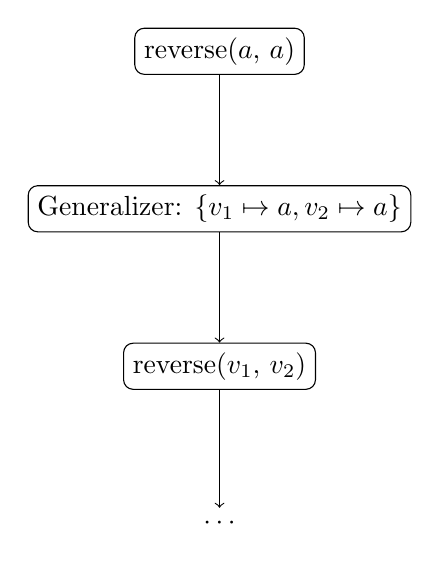
\begin{tikzpicture}[->,node distance=2cm, sibling distance=5cm]
                                                            
  \tikzstyle{conf}=[rectangle,draw, rounded corners=.8ex]

  \node[conf] (root) {\rel{reverse}($a$, $a$)} ;
  \node[conf] (gen) [below of = root] {Generalizer: $\{ v_1 \mapsto a, v_2 \mapsto a \}$};
  \node[conf] (node) [below of = gen] {\rel{reverse}($v_1$, $v_2$)};
  \node (rest)[below of = node] {$\cdots$};
   \path (root) edge (gen)
         (gen) edge (node)
         (node) edge (rest);
  % \path (root) edge node[above left,pos=1] {$\{a \mapsto \text{Zero}\}$} (childLeft)
  %       (root) edge node[above right,pos=1]{$\{a \mapsto \text{Succ}(a_1)\}$}(childRight)
  %       (childLeft) edge (left)
  %       (childRight) edge (childRight2)
  %       (childRight2) edge[bend right=90] (root);
\end{tikzpicture}
\caption{Демонстрация потери информации при обобщении вверх.}
\label{fig:genup}
\end{figure}
\todo{пояснения к примеру}

В случае же, когда обощение происходит на сам корень дерева, теряется эффект протягивания
констант.
